%!TEX root = ../Thesis.tex
\chapter{Cases}\label{cha:cases}
This chapter introduces the different cases this thesis looks into. 

\section{Pelton needles}\label{sub:pelton_needles}
    As mentioned, there was data available from two different power plants with pelton turbines controlled in a similar maner. One of plants had recorded several issues with the needle control, and was used as a case to test early detection of problems with the needle operation. 
    
    \begin{figure}
        \centering
        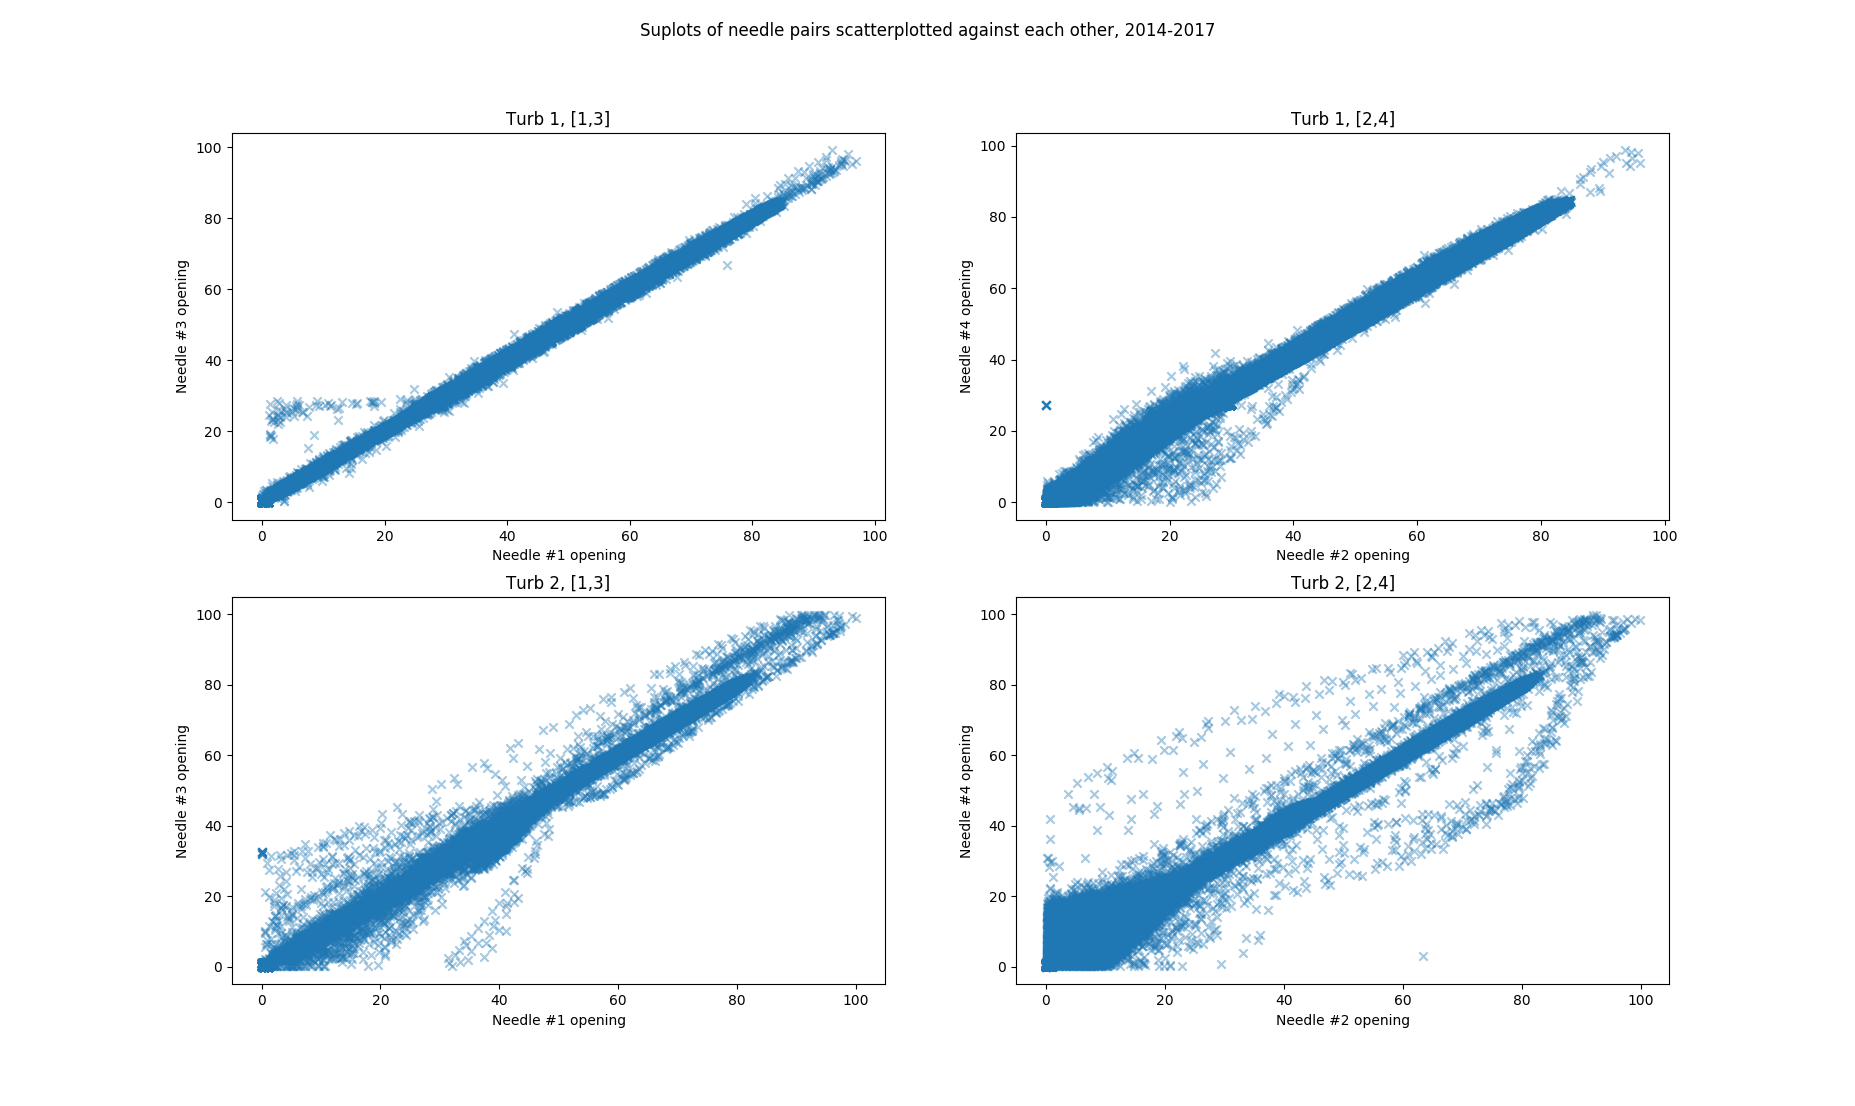
\includegraphics[width=\textwidth]{report/figures/analysis/hjartdola/hjar_scatterplot_all_needels.png}
        \caption{Caption}
        \label{fig:my_label}
    \end{figure}
    
    
    \begin{figure}
        \centering
        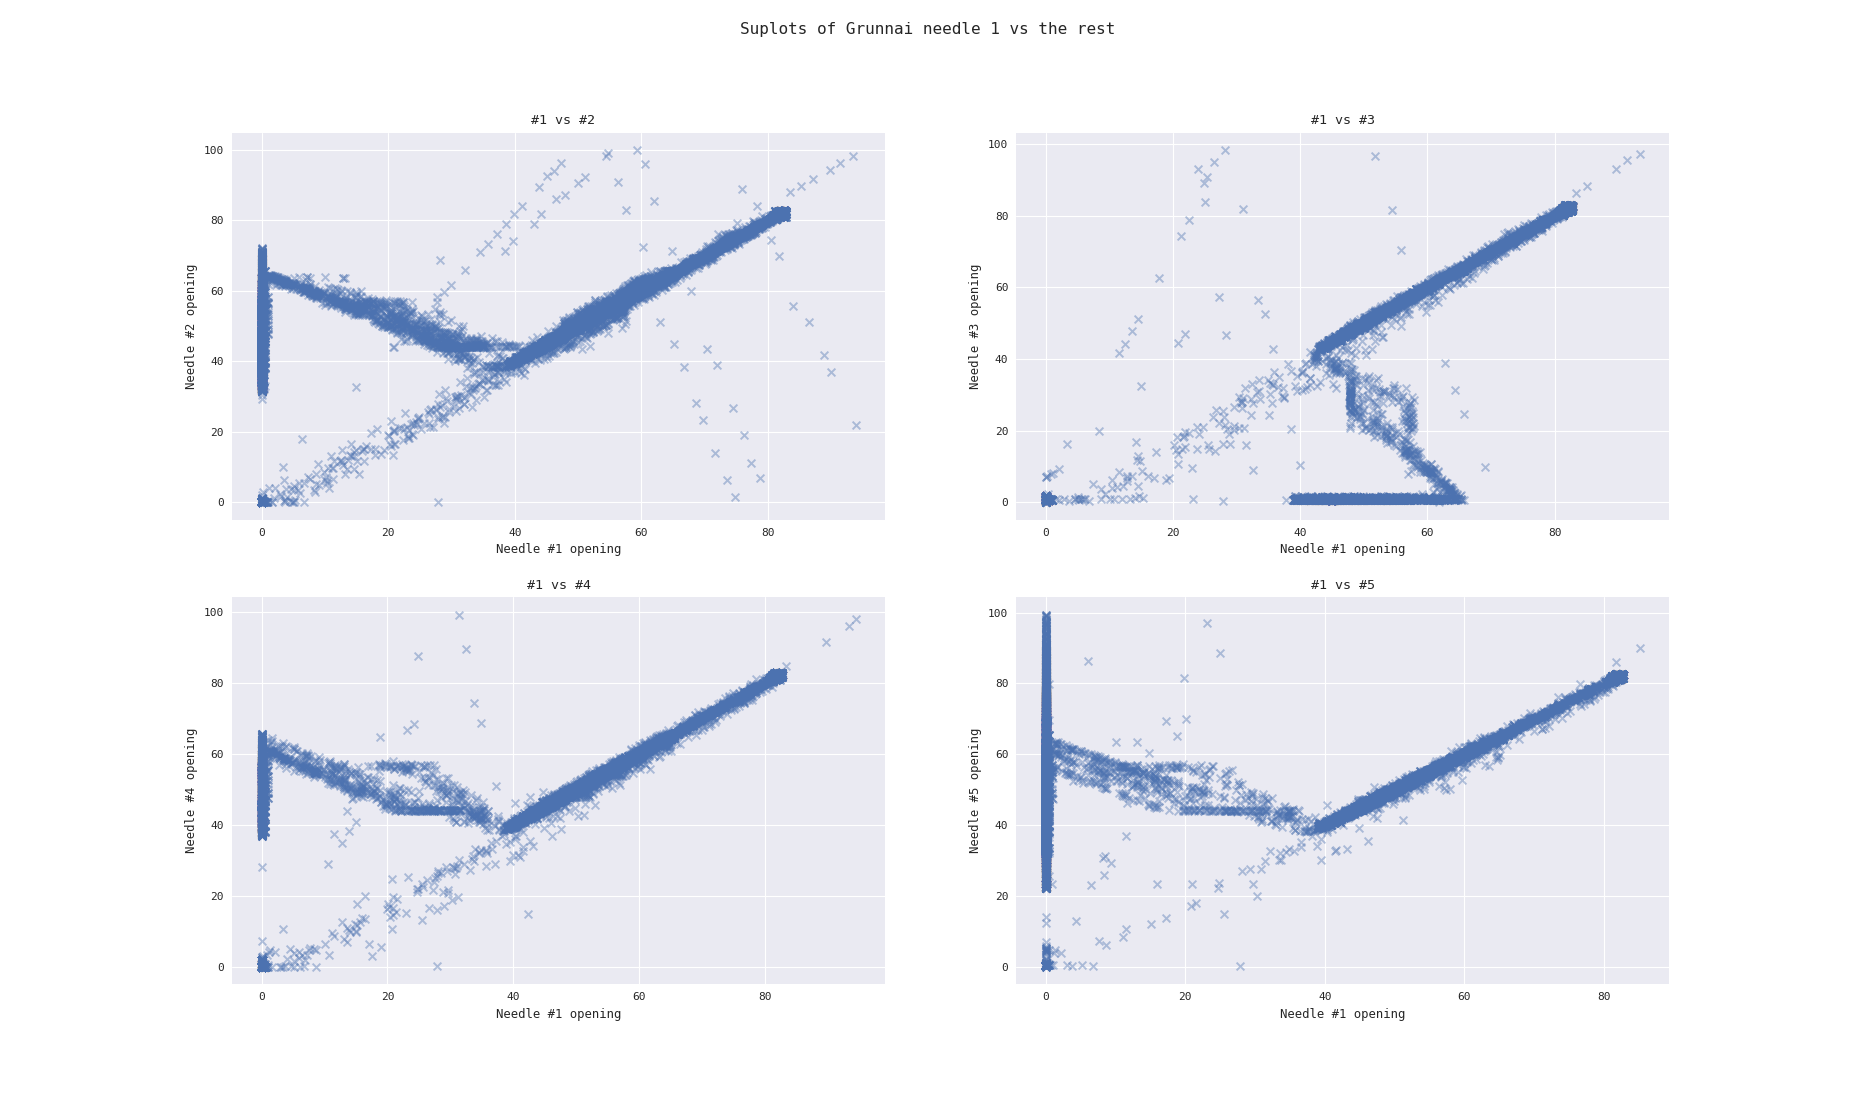
\includegraphics[width=\textwidth]{report/figures/analysis/grunnai/grun_scatterplot_1_vs_rest.png}
        \caption{Caption}
        \label{fig:my_label}
    \end{figure}
    
    
    \begin{figure}
        \centering
        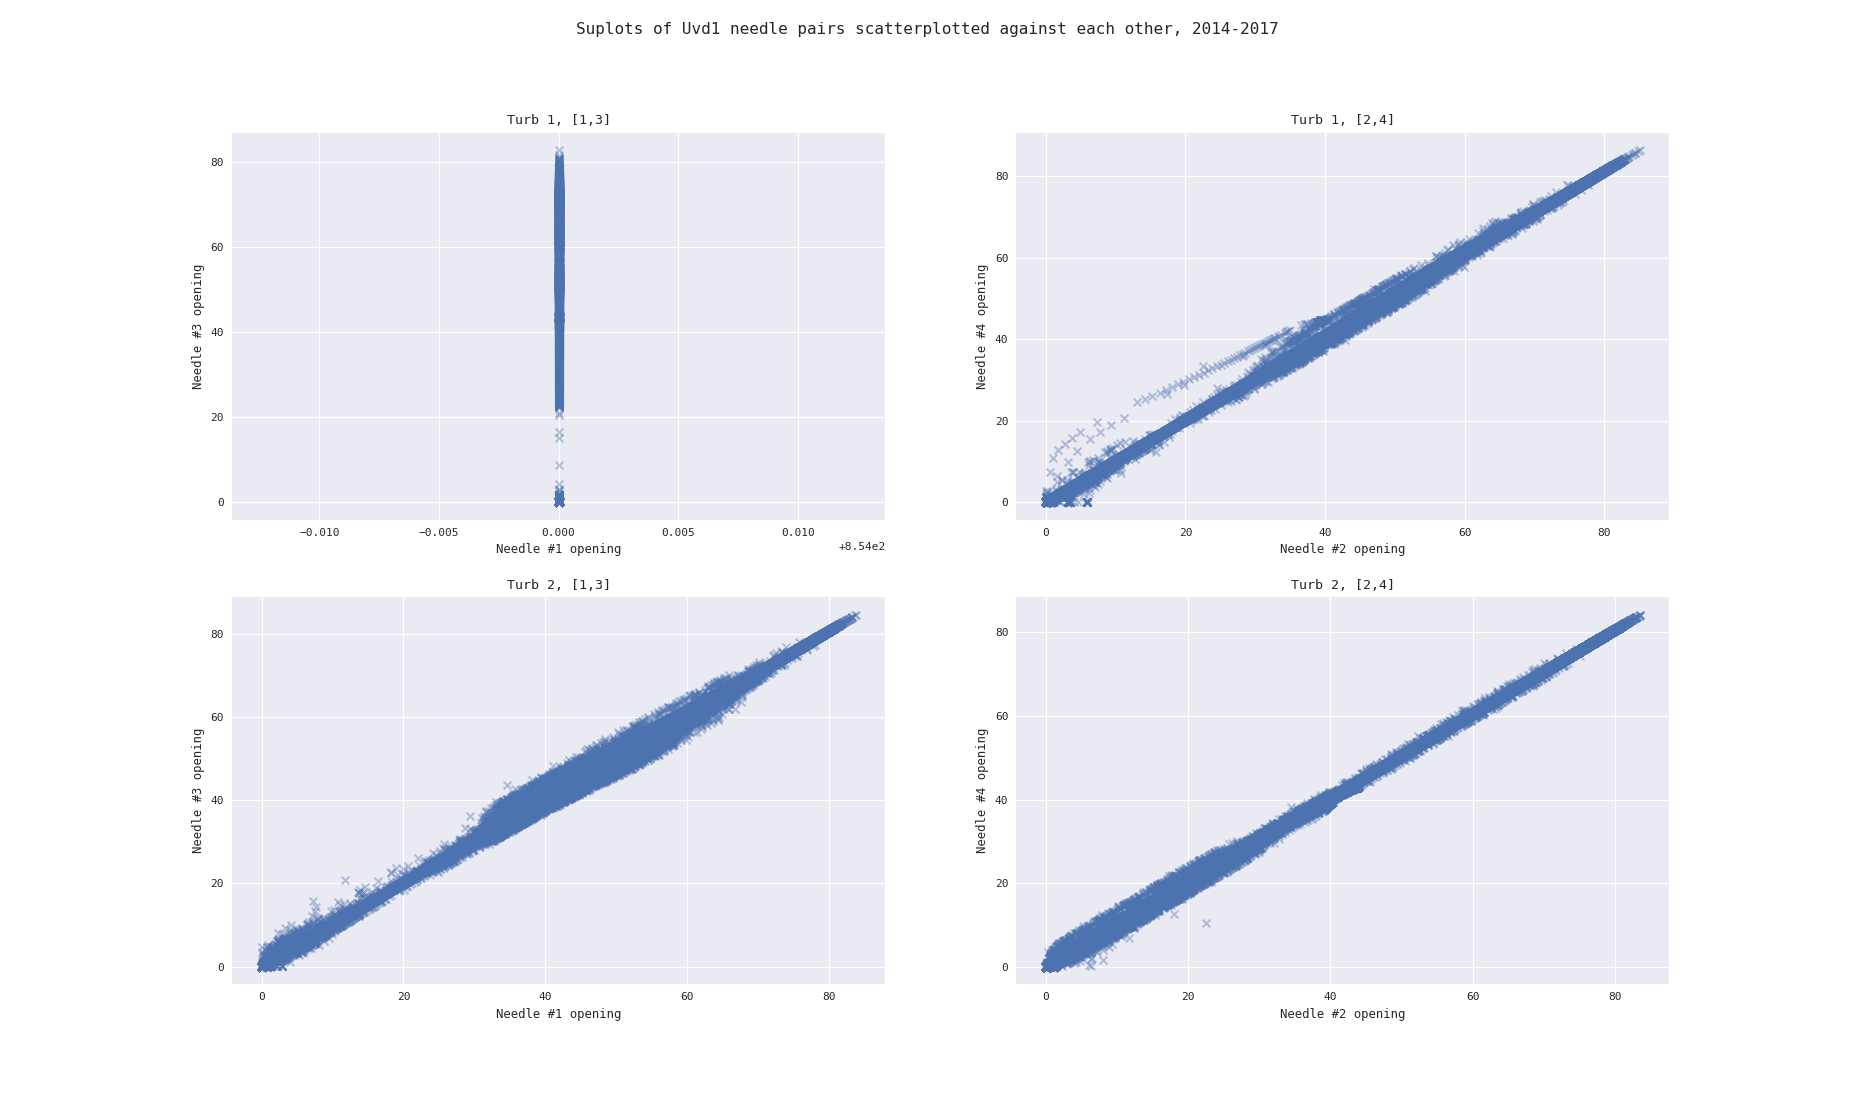
\includegraphics[width=\textwidth]{report/figures/analysis/uvdal1/uvd1_scatterplot_all_needels.png}
        \caption{Caption}
        \label{fig:my_label}
    \end{figure}
    
